\documentclass[final]{beamer}

\usepackage{amsthm}
\usepackage{algorithmic,algorithm}


\usepackage[scale=1.24]{beamerposter} % Use the beamerposter package for laying out the poster

\usetheme{confposter} % Use the confposter theme supplied with this template

\setbeamercolor{block title}{fg=ngreen,bg=white} % Colors of the block titles
\setbeamercolor{block body}{fg=black,bg=white} % Colors of the body of blocks
\setbeamercolor{block alerted title}{fg=black,bg=dblue!70} % Colors of the highlighted block titles
\setbeamercolor{block alerted body}{fg=black,bg=dblue!10} % Colors of the body of highlighted blocks
% Many more colors are available for use in beamerthemeconfposter.sty

%-----------------------------------------------------------
% Define the column widths and overall poster size
% To set effective sepwid, onecolwid and twocolwid values, first choose how many columns you want and how much separation you want between columns
% In this template, the separation width chosen is 0.024 of the paper width and a 4-column layout
% onecolwid should therefore be (1-(# of columns+1)*sepwid)/# of columns e.g. (1-(4+1)*0.024)/4 = 0.22
% Set twocolwid to be (2*onecolwid)+sepwid = 0.464
% Set threecolwid to be (3*onecolwid)+2*sepwid = 0.708

\newlength{\sepwid}
\newlength{\onecolwid}
\newlength{\twocolwid}
\newlength{\threecolwid}
\setlength{\paperwidth}{48in} % A0 width: 46.8in
\setlength{\paperheight}{36in} % A0 height: 33.1in
\setlength{\sepwid}{0.024\paperwidth} % Separation width (white space) between columns
\setlength{\onecolwid}{0.22\paperwidth} % Width of one column
\setlength{\twocolwid}{0.464\paperwidth} % Width of two columns
\setlength{\threecolwid}{0.708\paperwidth} % Width of three columns
\setlength{\topmargin}{-0.5in} % Reduce the top margin size
%-----------------------------------------------------------

\usepackage{graphicx}  % Required for including images

\usepackage{booktabs} % Top and bottom rules for tables

%----------------------------------------------------------------------------------------
%	TITLE SECTION 
%----------------------------------------------------------------------------------------

\title{Differentially Private ANOVA} % Poster title

\author{Zachary Campbell, Adam Groce, Anna Ritz, and Andrew Bray} % Author(s)

\institute{Reed College} % Institution(s)

%----------------------------------------------------------------------------------------

\begin{document}

\addtobeamertemplate{block end}{}{\vspace*{2ex}} % White space under blocks
\addtobeamertemplate{block alerted end}{}{\vspace*{2ex}} % White space under highlighted (alert) blocks

\setlength{\belowcaptionskip}{2ex} % White space under figures
\setlength\belowdisplayshortskip{2ex} % White space under equations

\begin{frame}[t] % The whole poster is enclosed in one beamer frame

\begin{columns}[t] % The whole poster consists of three major columns, the second of which is split into two columns twice - the [t] option aligns each column's content to the top

\begin{column}{\sepwid}\end{column} % Empty spacer column

\begin{column}{\onecolwid} % The first column

%----------------------------------------------------------------------------------------
%	OBJECTIVES
%----------------------------------------------------------------------------------------

\begin{alertblock}{Objectives}

Our goal is to apply methods of differential privacy to a common query framework used on biological and social-science databases. We set out to achieve the following:

\begin{itemize}
\item To formalize ANOVA in a differentially-private manner
\item Implement a differentially-private ANOVA algorithm 
\item To evaluate the performance of our algorithm with varying privacy parameters 
\end{itemize}

\end{alertblock}

%----------------------------------------------------------------------------------------
%	INTRODUCTION & MOTIVATION
%----------------------------------------------------------------------------------------

\begin{block}{Introduction \& Motivation}


The objects of concern in this project are statistical databases. We will think of these specifically as databases populated with individuals' private, sensitive information (such as medical records, financial records, genome sequences, etc.). Differential privacy is a mathematical formulation within the field of database privacy that aims to allow queries on a statistical database, while offering strong privacy guarantees. That is, when one asks for quantitative information from a database (think mean, median, etc.), we want to guarantee that this query will be executed in such a way that with high probability it does not leak any identifying information about individual records.

%\end{block}

%\begin{block}{Motivation}

It has been shown many times that simple anonymization of database records is not sufficient to protect the privacy of individuals who populate a database. Perhaps most famously, in \cite{narayanan2008robust}, researchers used anonymized and publicly available data released by Netflix, in addition to auxiliary databases, to identify specific users in the Netflix data. Similar attacks have shown effective on anonymized genetic data, leading to widespread data removal. The goal of differential privacy is to allow queries on these databases in such a way that privacy is guaranteed, no matter what auxiliary information an attacker might have. For another attack, see \cite{homer2008resolving}.

\end{block}

%----------------------------------------------------------------------------------------
%	Differential Privacy
%----------------------------------------------------------------------------------------

\begin{block}{Differential Privacy}

In the following, let $x$ and $y$ be databases in the universe $\mathcal{X}$. We define the notation $||x-y||_1$ to be a measure of how many records differ between databases $x$ and $y$. We formally define differential privacy as follows:
A randomized algorithm $\mathcal{M}$ with domain $\mathcal{X}$ is $\epsilon$-differentially private if for all $\mathcal{S}\subseteq \text{Range}(\mathcal{M})$ and for all $x,y \in\mathcal{X}$ such that $||x - y||_1 \leq 1$:

\[
\text{Pr}[\mathcal{M}(x) \in \mathcal{S}] \leq \exp(\epsilon) \text{Pr}[\mathcal{M}(y) \in \mathcal{S}].
\]

In general, privacy is acheived by injecting random noise into the data. For more information see \cite{dwork2014algorithmic}

%\begin{figure}
%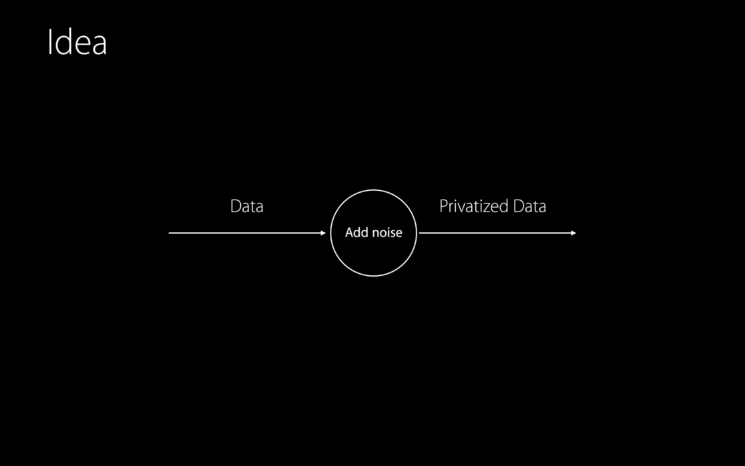
\includegraphics[width=1.0\linewidth]{diffpriv.png}
%\caption{In general, privacy is acheived by injecting random noise into the data. For more information 
%	see \cite{dwork2014algorithmic}}
%\end{figure}

\end{block}


%----------------------------------------------------------------------------------------

\end{column} % End of the first column

\begin{column}{\sepwid}\end{column} % Empty spacer column

\begin{column}{\twocolwid} % Begin a column which is two columns wide (column 2)

\begin{columns}[t,totalwidth=\twocolwid] % Split up the two columns wide column

\begin{column}{\onecolwid}\vspace{-.6in} % The first column within column 2 (column 2.1)

%----------------------------------------------------------------------------------------
%	ANOVA
%----------------------------------------------------------------------------------------

\begin{block}{ANOVA}

The setting is that we have a dataset that can be partitioned into $k$ disjoint groups of 
individuals, based on some categorical predictor variable. The goal of an analysis of variance, or ANOVA, is to test if there is astatistical difference between the means of these groups. 
We now define the specifics of an ANOVA test.
Let $\textbf{D}$ be our database, and let $\{D_i \; |\; 1\leq i\leq k \}$ be a partition of 
$\textbf{D}$, where each $D_i$ is what we think of as a ``group.'' We denote the $j$th entry of group $i$ by $y_{ij}$, the mean of group $i$ by $\overline{y}_i$, and the mean of the entire 
database by $\overline{y}$. Also, let $x_i = |D_i|$. 
There are two important measures in the ANOVA framework that we will use:
\[
\text{SSA} = \sum_{i=1}^{k} x_i(\overline{y}_i - \overline{y})^2,
\]
\[
\text{SSE} = \sum_{i=1}^{k} \sum_{j=1}^{x_i} (y_{ij} - \overline{y}_i)^2.
\]

{\color{red}{SENTENCES HERE ABOUT MSA, MSE AND F}}

\end{block}
%---------------------------------------------------------------------------------------


%----------------------------------------------------------------------------------------

\end{column} % End of column 2.1

\begin{column}{\onecolwid}\vspace{-.6in} % The second column within column 2 (column 2.2)

%----------------------------------------------------------------------------------------
%	OUR ALGORITHM
%----------------------------------------------------------------------------------------

\begin{block}{Our Algorithm}
Our algorithm uses a technique called the Laplace mechanism, which is a powerful primitive in 
differential privacy. The idea is, given a query $f:\mathcal{D}\to\mathbb{R}^{k}$, we first analyze the sensitivity of $f$, denoted $\Delta f$. Intuitively, the sensitivity captures how much the output of our function can change for a change of input in a specified range. Using this sensitivity, we then draw noise from the Laplace distribution $\text{Lap}(\Delta f / \epsilon)$.

\begin{figure}
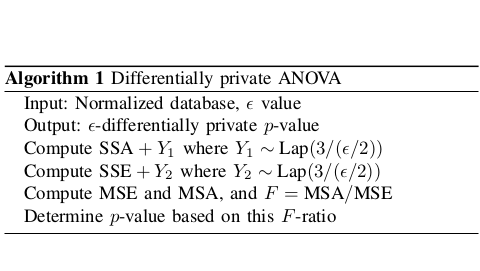
\includegraphics[width=1.0\linewidth]{algorithm.png}
%\caption{Our algorithm, which adds Laplacian noise based on the provable sensitivity of 
%	general sum-of-squares formulas, and returns a differentially-private $p$-value.}
\end{figure}

\end{block}

%----------------------------------------------------------------------------------------

\end{column} % End of column 2.2

\end{columns} % End of the split of column 2 - any content after this will now take up 2 columns width

%----------------------------------------------------------------------------------------

%\begin{columns}[t,totalwidth=\twocolwid] % Split up the two columns wide column again

%\begin{column}{\onecolwid} % The first column within column 2 (column 2.1)


%\end{column} % End of column 2.1

%\begin{column}{\onecolwid} % The second column within column 2 (column 2.2)

%----------------------------------------------------------------------------------------
%	RESULTS
%----------------------------------------------------------------------------------------

\begin{block}{Results}

Our results indicate that one can carry out an ANOVA test on reasonable database sizes with 
reasonable privacy guarantees. 

\begin{center}
\begin{figure}
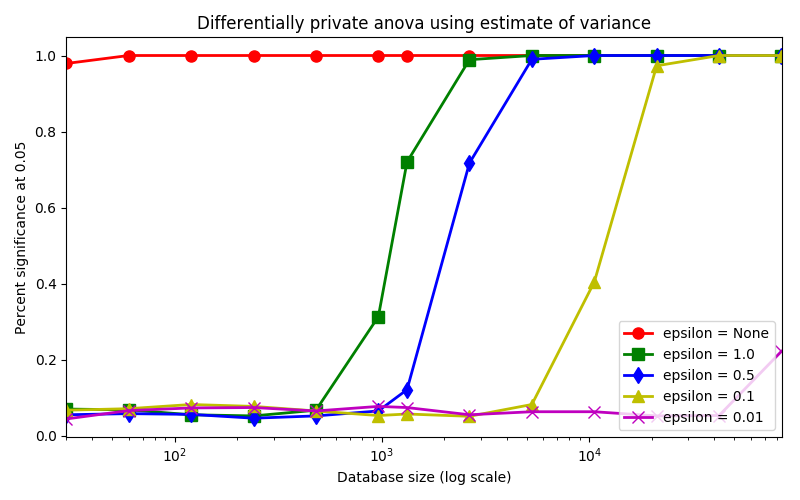
\includegraphics[width=.85\linewidth]{varest1000_1.png}
%\caption{Differentially-private ANOVA with varying database sizes and epsilon values.}
\end{figure}
\end{center}

\end{block}

%----------------------------------------------------------------------------------------

%\end{column} % End of column 2.2

%\end{columns} % End of the split of column 2

\end{column} % End of the second column


\begin{column}{\sepwid}\end{column} % Empty spacer column

\begin{column}{\onecolwid} % The third column

%----------------------------------------------------------------------------------------
%	CONCLUSION
%----------------------------------------------------------------------------------------

\begin{block}{Conclusion}

We show that for reasonable database sizes, one can execute differentially-private ANOVA 
tests with reasonable privacy guarantees, without significant loss in accuracy. Of course,
the model is not as accurate as when using non-private ANOVA, but that is the trade-off. As 
database size increases, the output of the differentially-private algorithm converges to 
the output of the non-private algorithm. Ultimately, we have shown that differentially-private ANOVA maintains strong utility.

\end{block}

%----------------------------------------------------------------------------------------
%	FURTHER WORK
%----------------------------------------------------------------------------------------

\begin{block}{Further Work}

This project is only a small step into what is a very large area for exploration. There are 
certainly ways to get tighter bounds on the sensitivity of the sum-of-squares measurements, 
which would improve accuracy. We did make some attempt at implementing more complicated 
methods, but they require further work.

\end{block}

%----------------------------------------------------------------------------------------
%	REFERENCES
%----------------------------------------------------------------------------------------

\begin{block}{References}

\bibliographystyle{abbrv}
\bibliography{sample}

\end{block}

%----------------------------------------------------------------------------------------

\end{column} % End of the third column

\end{columns} % End of all the columns in the poster

\end{frame} % End of the enclosing frame



\end{document}

